\documentclass[a4paper,12pt]{article}

\usepackage[T1]{fontenc}
\usepackage[utf8]{inputenc}
\usepackage{listings}
\usepackage{hyperref}
\usepackage{xcolor, graphicx}

\title{Exercise 1,  MATLAB Environment Lab}
\author{Linnéa Olsson, André Frisk, Andreas R Almgren}

\begin{document}

\maketitle

\section{Abstract}

This laboratory reports main focus lies within getting us familiar with the MATLAB environment. This is achieved through asking us to write a script that outputs a graph. 

\section{Introduction}

In this laboratory report we are going to use MATLAB to create a graph. MATLAB is a language that manipulates vectors and matrices. This lab is mostly about learning how to work with MATLAB and see the benefits of using it. 

\subsection{Purpose}
\label{Purpose}

The purpose of this lab is to plot the function $\sin(10x) + x$ in blue colour, $\sin(30x) + 1$ in red colour and $x^{2}$ in green colour. The plotted graph is meant to have smooth curves and dotted grids; have the range $(-1,5)$ and domain $[0,2]$ - and also have labels for its axes: $x$-axis as $x$ and $y$ as $f(x)$.

\section{Method}
\subsection{Tools/Material}

\begin{itemize}
    \item {\setlength{\parindent}{0cm}
          A computer fitting for the task
          }
    \item $\LaTeX$ editor, in this lab Overleaf was used
    \item MATLAB
    \item  EX1\_perspective.zip (\href{https://hh.blackboard.com/bbcswebdav/pid-211495-dt-content-rid-1644398_1/xid-1644398_1}{\color{blue}{link}})
\end{itemize}

\subsection{Implementation}

{\setlength{\parindent}{0cm}
We opened Matlab and entered the following code:
}

\\

\iffalse
Sorry for the ugly formatted code down below, it looks better in the m-file e1_1.m.
\fi

\begin{lstlisting}
% Line in remarks: Linnea Olsson, Andre Frisk, Andreas R Almgren
% Create a vector of 1000 evenly spaced points in the interval [0, 2]. 
x = linspace(0, 2, 1000); 
f1 = sin(10 * x) + x;
f2 = sin(30 * x) + 1;
f3 = x.^2; 
% Plot the functions f1, f2 and f3. Specify the colours of respective 
% functions.
plot(x, f1, 'b', x, f2, 'r', x, f3, 'g') 
% Specify limits on f-axis.
ylim([-1 5])
% Specifies axis tick values.
xticks([0 0.2 0.4 0.6 0.8 1 1.2 1.4 1.6 1.8 2]) 
% Set label below x-axis.
xlabel('x') 
ylabel('f(x)') 
grid on 
% Current axes.
ax = gca; 
% Set the style of the gridlines to be dotted.
ax.GridLineStyle = '--'; 
% Make a legend.
legend('sin(10x) + x','sin(30x) + 1', 'x^2', 'Location', 'northeast') 
% Save plot as a PNG named e1_1. 
print('-dpng', '-r600', 'e1_1') 
\end{lstlisting}

\\

{\setlength{\parindent}{0cm}
After having finished the code, we ran it.
}

\newpage

\section{Result}

We found that when executing the file e1\_1.m, we got the output that can be seen in figure \ref{Graph}.

\begin{figure}[h!]
\centering
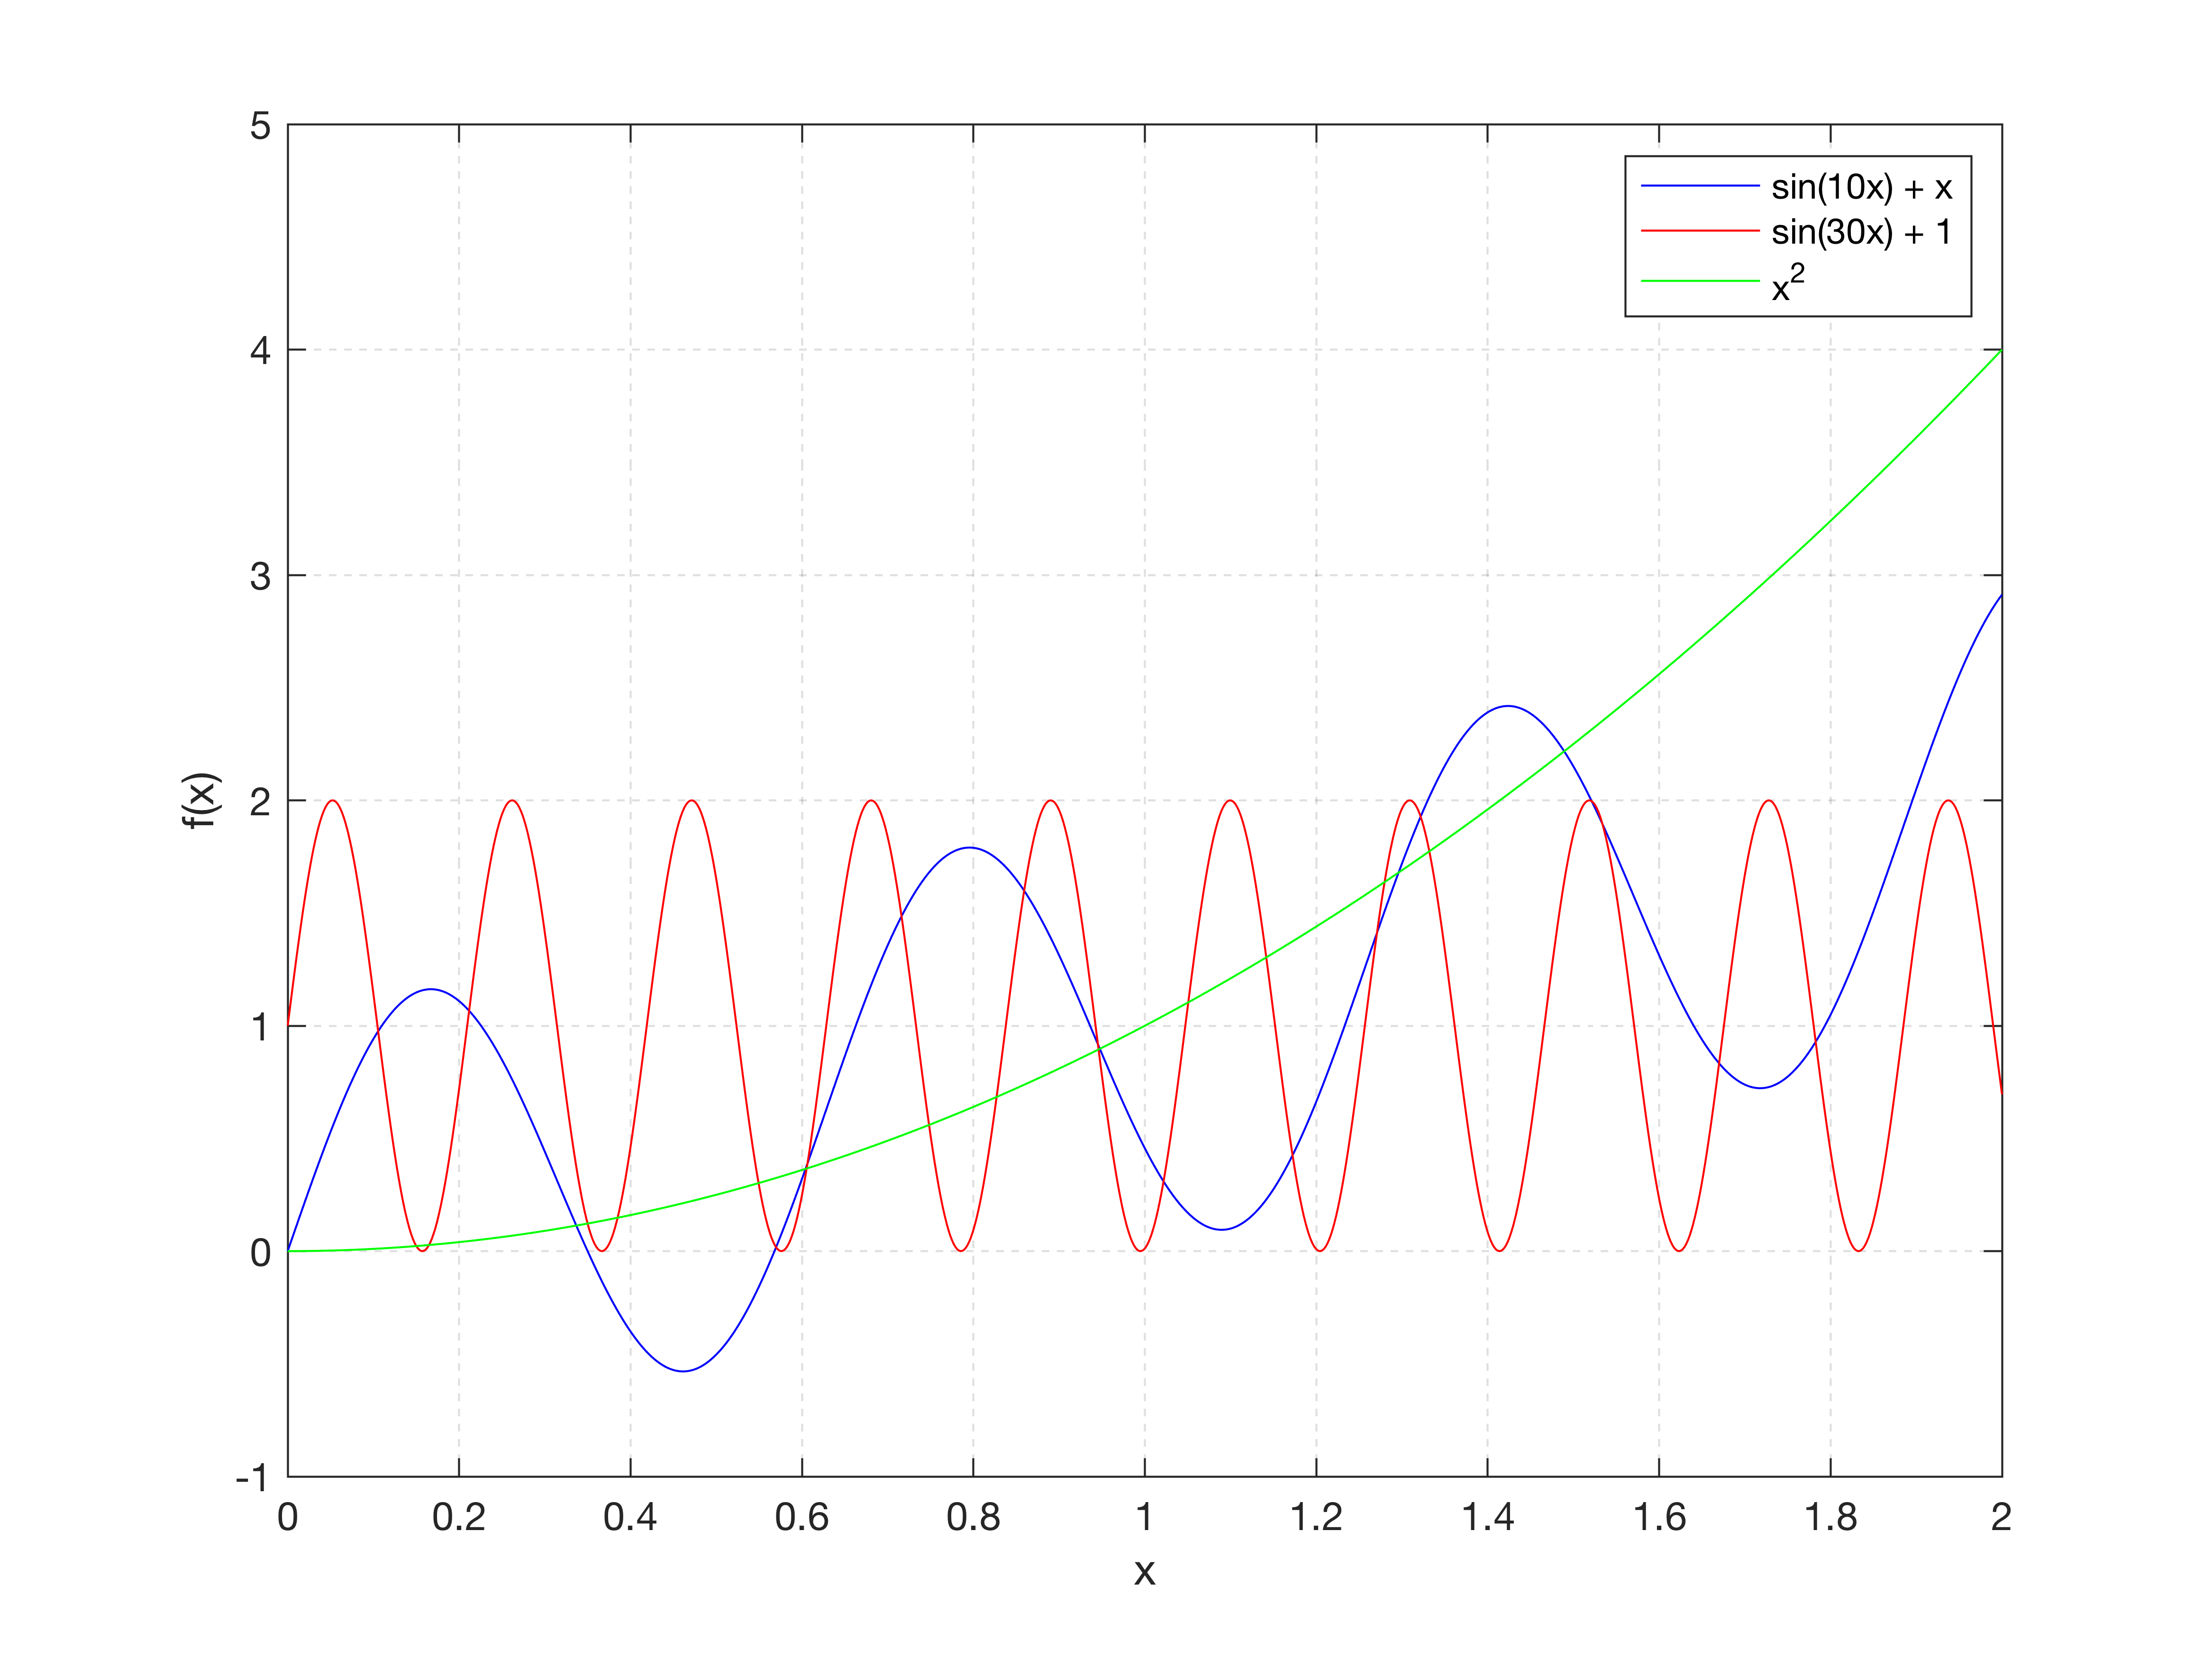
\includegraphics[width=\textwidth]{e1_1.png}
\caption{Output of e1\_1.m. }
\label{Graph}
\end{figure}

{\setlength{\parindent}{0cm}
Figure \ref{Graph} has the functions $\sin(10x) + x$, $\sin(30x) + 1$ and $x^{2}$ plotted in it. 
}

\section{Conclusion}

We successfully plotted a graph including what we aimed to include in \ref{Purpose}.

\section{Note on a bug in the instructions}

In the pdf e1v3.pdf (found in EX1\_perspective.zip) we are told to plot the function $\sin(30x) + 1$ in red and also that the same function should be plotted in green. We chose to use the first alternative. 

\end{document}
